\chapter{QUIC协议的原理分析}

\label{cha:analysis}
本章将详细介绍一下QUIC协议的优点及其对应的实现原理,包括QUIC协议的连接建立过程(包括握手方式及内容、连接的建立方式),对出现丢包情况下的特殊处理方式,出现拥塞时采取的拥塞控制算法,两种类型的流控算法以及其他有用的特性。
\section{QUIC优点}
正如第\ref{cha:intro}章中所描述的,QUIC的主要优点有以下五点。
\begin{itemize}
  \item 低连接延迟
  \item 更好的拥塞控制算法选择
  \item 多路复用流来避免线头阻塞
  \item 前向纠错算法
  \item 连接迁移功能
\end{itemize}
\subsection{低连接延迟}
低连接延迟是由于QUIC与TCP+TLS有着不同的握手过程,并不需要三次握手,同时在握手过程中附带了加密信息,从而不需要进行TLS额外的加密握手过程,所以相比于TCP会有更少的传输延迟。QUIC不仅在建立连接成功之后有与TCP+TLS的时延更少,在第一次建立连接的时候也比TCP+TLS的时延更少。 具体的QUIC连接过程参考本章对QUIC连接建立流程的描述。图\ref{fig:quicvstcp}体现了QUIC与TCP+TLS在传输过程中的时延对比,包括初次建立连接和成功建立连接之后的传输。
\begin{figure}
  \centering
  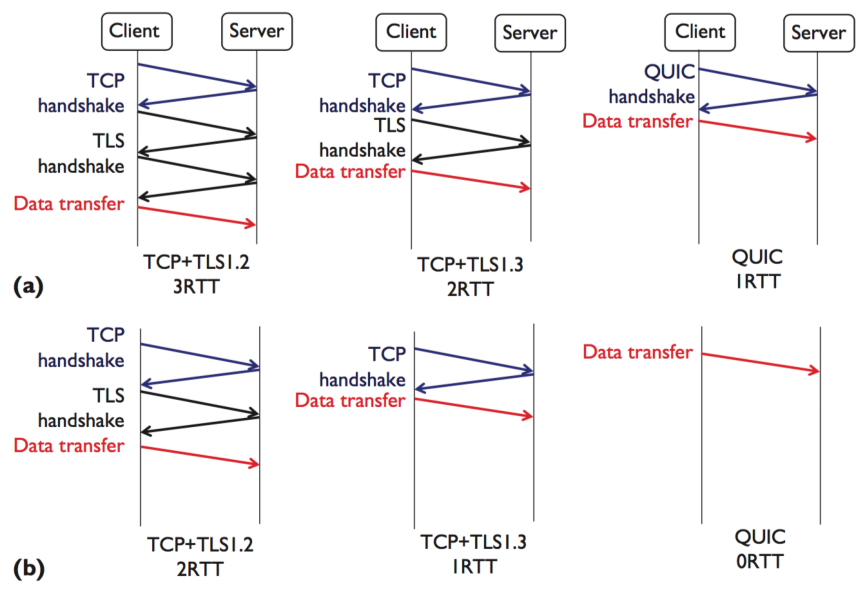
\includegraphics[width=\textwidth]{quicvstcp}
  \caption{TCP+TLS与QUIC握手延时(a)为首次连接(b)为连接成功后情形}
  \label{fig:quicvstcp}
\end{figure}

\section{QUIC原理简介}
\subsection{传输格式}
QUIC的传输格式是QUIC很多原理实现的基础,同时又考虑到整个QUIC协议的传输格式的复杂性,因此在这部分列出了QUIC包传输格式中较为重要的一部分内容来帮助后面的原理分析。QUIC的包由公共包头加上加密后的一系列帧构成,下面将主要介绍公共包头的主要组成部分和几种比较重要的帧。
\subsubsection{公共包头}
公共包头的主要组成部分如下
\begin{itemize}
  \item 连接ID
  \item QUIC版本号
  \item 包号
\end{itemize}
连接ID是一个由客户端选择的无符号的64位静态随机数,它来标示一种连接。因为QUIC的连接被设计成即便是短暂断开依然能保持在连接状态,所以这个连接ID能够使QUIC在网络连接的IP改变之后依然能迅速回到已有的连接状态中,即使得QUIC协议具有很好的移动性。

QUIC版本号在连接建立过程中起到重要的作用,因为QUIC协议在不断的更新,需要在客户端和服务端之间有统一的QUIC协议接口,QUIC版本号会提供若干个供支持的版本号,从而使协议能够顺利运行。

包号是独一无二而且一直单调增加的,即便是出现丢包重传的情况,包序号也会不断增加,这种特性避免了TCP中出现的重传包时ACK包的歧义性问题,本章后部分会具体分析包序号与丢包重传相关的算法。
\subsubsection{重要的帧}
\begin{itemize}
  \item Stream帧
  \item ACK帧
  \item Stop\_Waiting帧
\end{itemize}
Stream帧是用来控制流传输的,Stream帧的存在每个Stream帧中都会含有传输的流的ID,还有一些关于流是否传输完毕的标识。Stream帧中会包括具体的数据内容。

ACK帧是用来接收方用来通知发送端哪些包已经成功接收(被ACK),而哪些包丢失了,这些丢失的包可能通过一定方法恢复也可能需要重传。ACK帧中包含了1到256个ACK块,这些ACK块是已经确认的包的范围。

Stop\_Waiting帧是用来辅助进行ACK的一个帧。发送端会周期性发送Stop\_Waiting帧,来通知接收方不必要再去确认小于特定序列号的包(这些包可能已经由发送方以新的序列号重传),从而减少了需要进行ACK的包的个数。

\subsection{连接建立}
QUIC连接是由客户端发起的,流程的描述和流程图表示如下。
\begin{figure}
  \centering
  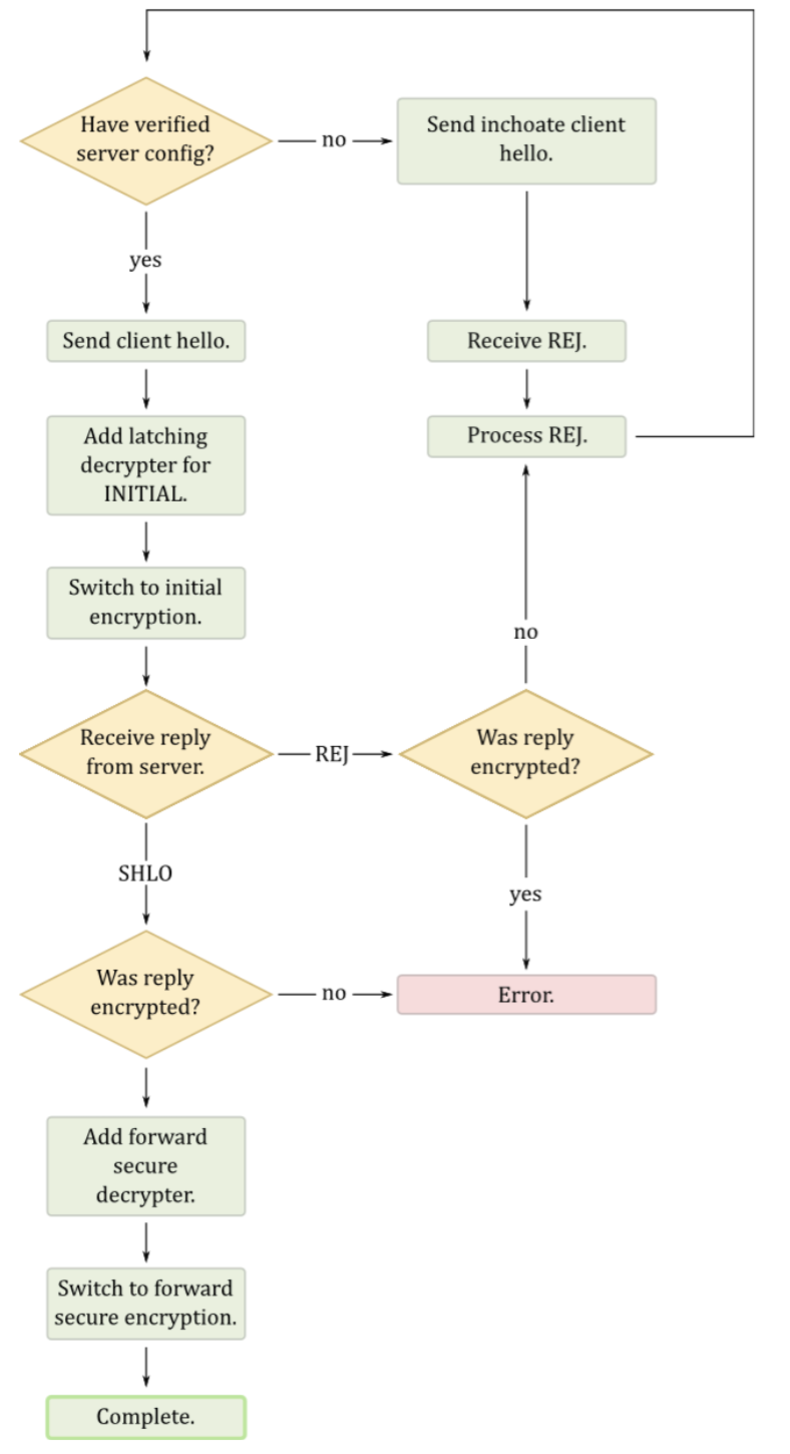
\includegraphics[width=0.5\textwidth]{quicHandShake}
  \caption{客户端握手流程}
  \label{fig:quichandshake}
\end{figure}
\begin{itemize}
  \item[1.] 客户端判断本地是否已有服务器的配置信息,如果有则跳转到第5步,否则继续。
  \item[2.] 客户端向服务器发送空的客户端hello消息(CHLO),并请求服务器回传配置信息。
  \item[3.] 服务端受到CHLO消息后,回复给客户端拒绝消息(REJ),并在其中附带自己的配置信息
  \item[4.] 客户端收到服务端发送来的REJ消息之后,存储服务端的配置信息,并回到第1步。
  \item[5.] 客户端向服务端发送完整的客户端hello消息,并开始正式握手,在这次的hello消息中将会包括加密连接的一些信息。
  \item[6.] 服务端受到完整CHLO信息后,如果不同意连接就回复拒绝消息(REJ),则同第3步的操作;如果同意连接则连接成功,服务端回复服务端hello信息(SHLO),并在其中包括成功加密的信息。
  \item[7.] 客户端接受服务端的信息,如果是REJ信息,则同第4步操作;如果是SHLO消息,则继续进行加密信息的交换。
  \item[8.] 根据沟通成功的密钥进行通信,握手成功。
\end{itemize}

\subsection{丢包处理}
QUIC在处理丢包主要有两种方案。
\begin{itemize}
  \item 前向纠错算法
  \item 丢包重传
\end{itemize}
\subsubsection{前向纠错算法}
前向纠错算法是通过在传输的包中添加冗余信息,来进行数据的校验和恢复,从而实现丢包的恢复,避免进行重传。在QUIC中,主要使用的前向纠错算法是异或算法(XOR)。这种异或算法的基本做法是将若干个包作为一组,额外添加一个冗余的异或包,这样便可以实现只要任何一个包丢失,都可以通过该异或包恢复出结果。这种异或算法的优点是计算成本低而且容易实现,而缺点是只能允许一组包里面有一个丢包出现,否则就不能恢复。
\subsubsection{丢包重传}
丢包重传是TCP在遇到丢包时选择的办法,在QUIC不能使用前向纠错算法进行丢包恢复的时候,也会使用丢包重传来进行恢复,在这一部分将主要介绍QUIC使用的丢包重传算法,以及分析它与TCP的不同之处。
首先在QUIC的传输格式中,与丢包恢复相关联的帧有两个,一是Stream帧,因为Stream帧包含了应用的数据;二是ACK帧,包含了连接过程中传输数据时交互的确认信息。在QUIC中,发送方会设置一个重传计时器,计时器的设置与TCP相似;在收到ACK包之后(包括了最大已被确认的包序号X),会忽略已经被接受放确认的包(即这些包的传输成功),并根据包中携带的时间戳来更新重传计时器的设置。把那些编号小于X并且没有被NACK的包记为ACK,而对于那些编号小于X并且被NACK的包计入丢包计数器,在丢包计数器超过一定阈值之后,则会认定该包丢失,选择进行重传。与TCP的重传机制相比较,即便是重传的包,都会有恒定增加的包序号,从而避免了TCP中会出现的ACK包的歧义性。此外,在QUIC中有更多的ACK块,从而能使得QUIC在高丢包的环境下加快传输的速度,这一点在\ref{cha:evaluation}的实验结果中可以非常清晰的看到。
\subsection{拥塞控制}

\subsection{流控算法}

\section{QUIC相关原语及接口整理}
\subsection{Quic\_server}
\subsection{Quic\_client}
\section{本章小结}
